\subsubsection*{Figures and tables for EXP2 (Section~\ref{sec:results-P})}

\begin{figure}[H]
    \centering
    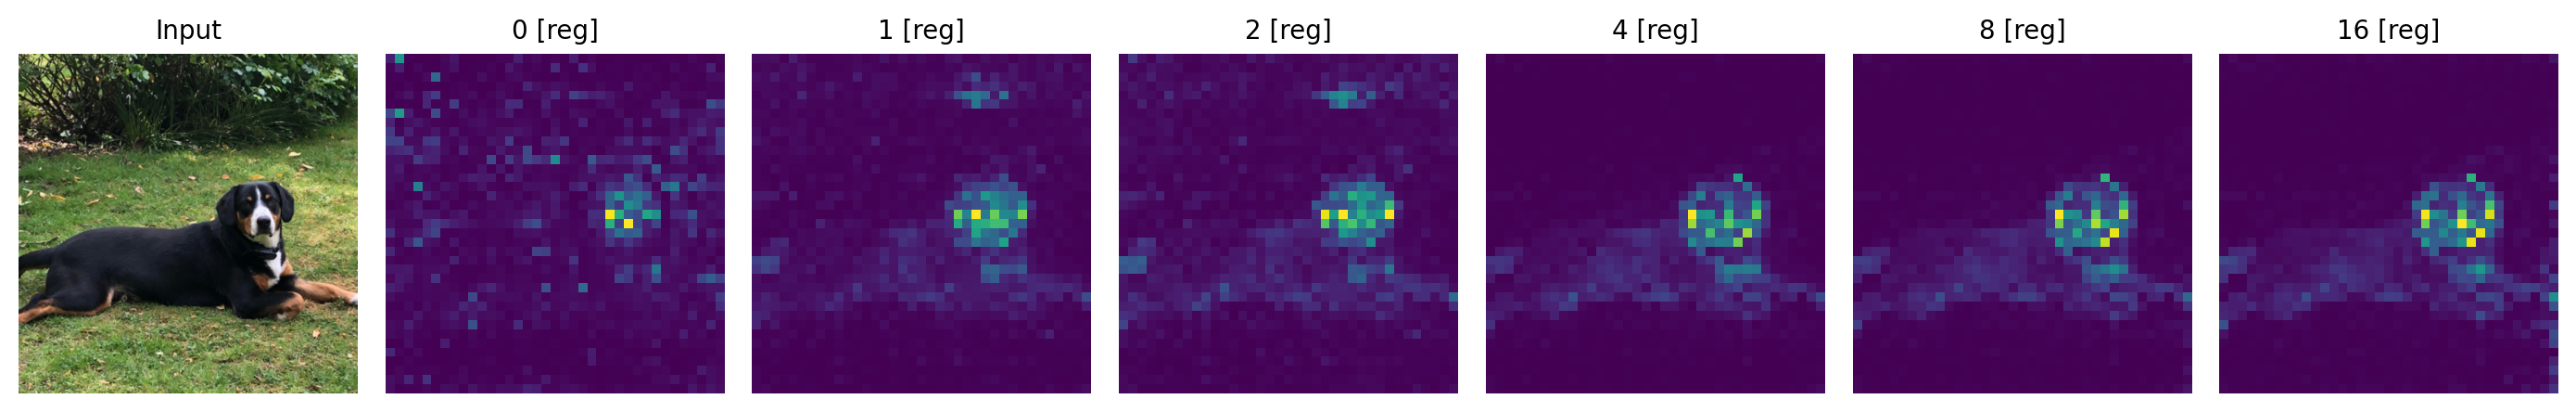
\includegraphics[width=0.95\linewidth]{../../src/Paolo/results/figure8_top/figure8_top.png}\\[2pt]
    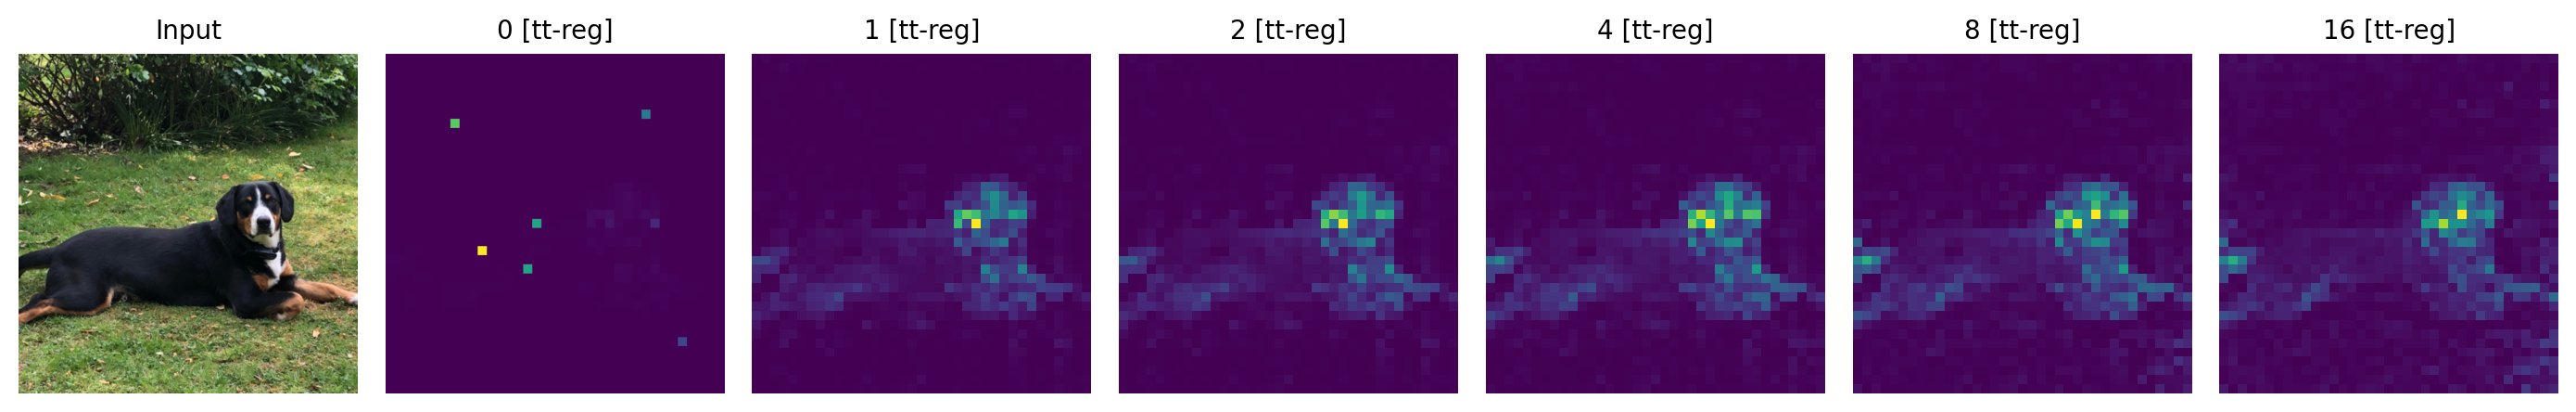
\includegraphics[width=0.95\linewidth]{../../src/Paolo/results/figure8_top_ttreg/figure8_top_ttreg.png}\\[2pt]
    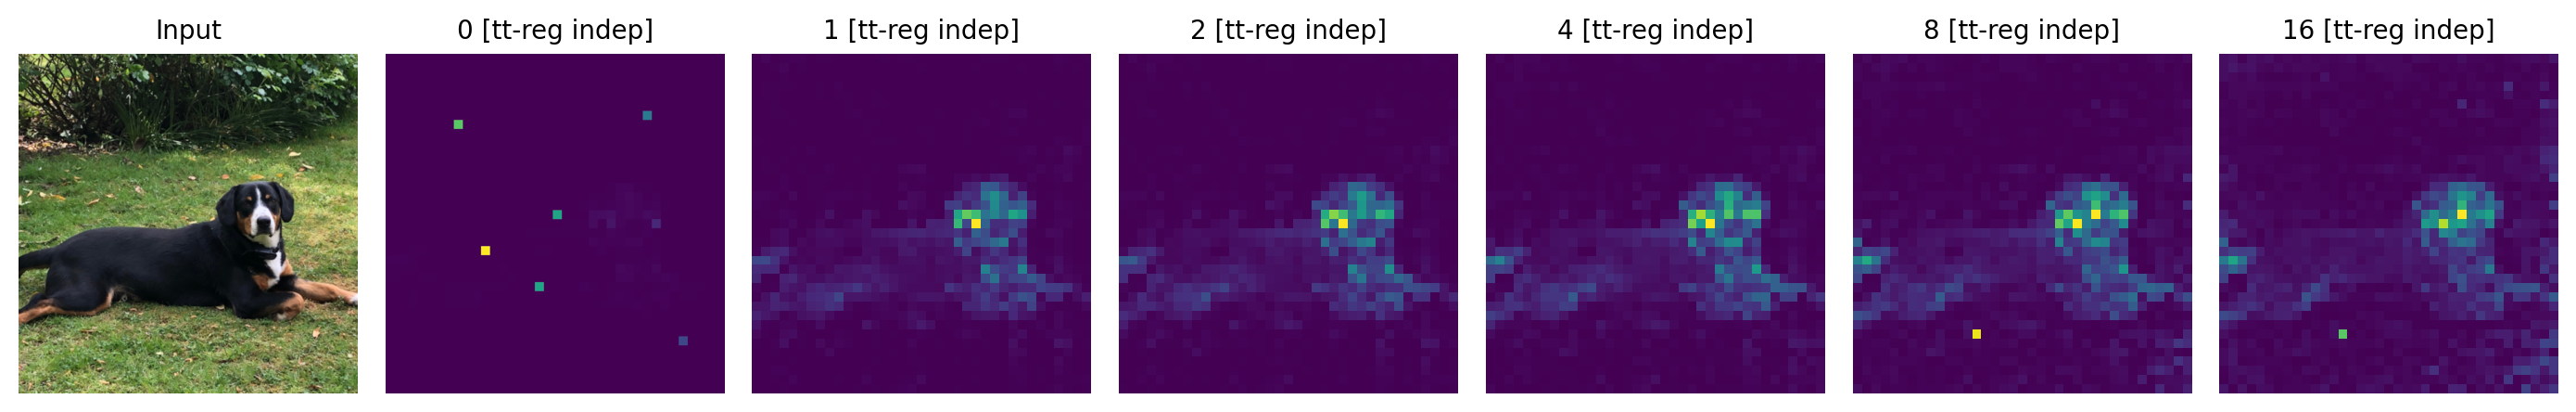
\includegraphics[width=0.95\linewidth]{../../src/Paolo/results/figure8_top_ttreg_indep/figure8_top_ttreg_indep.png}
    \caption{Attention maps of the last self-attention layer (CLS$\to$patch) for $N\in\{0,1,2,4,8,16\}$ register tokens on DINOv2 ViT-L/14. \textbf{Row 1}: truncate/cycle proxy on DINOv2-reg4 -- maps are noisy for $N<4$ because the model expects exactly four registers, and the artifact channels diffuse over the patches when no slot is available. \textbf{Row 2}: Jiang test-time registers on the no-register DINOv2 baseline -- the single isolated outlier visible at $N=0$ is absorbed by the first register and the map cleans up. \textbf{Row 3}: our independent variant in which the top-$N$ distinct outlier values are distributed across the $N$ test-time registers rather than duplicated -- maps clean up from $N=1$ but a small residual hotspot reappears at $N=8,16$.}
    \label{fig:f8-top}
\end{figure}

\begin{figure}[H]
    \centering
    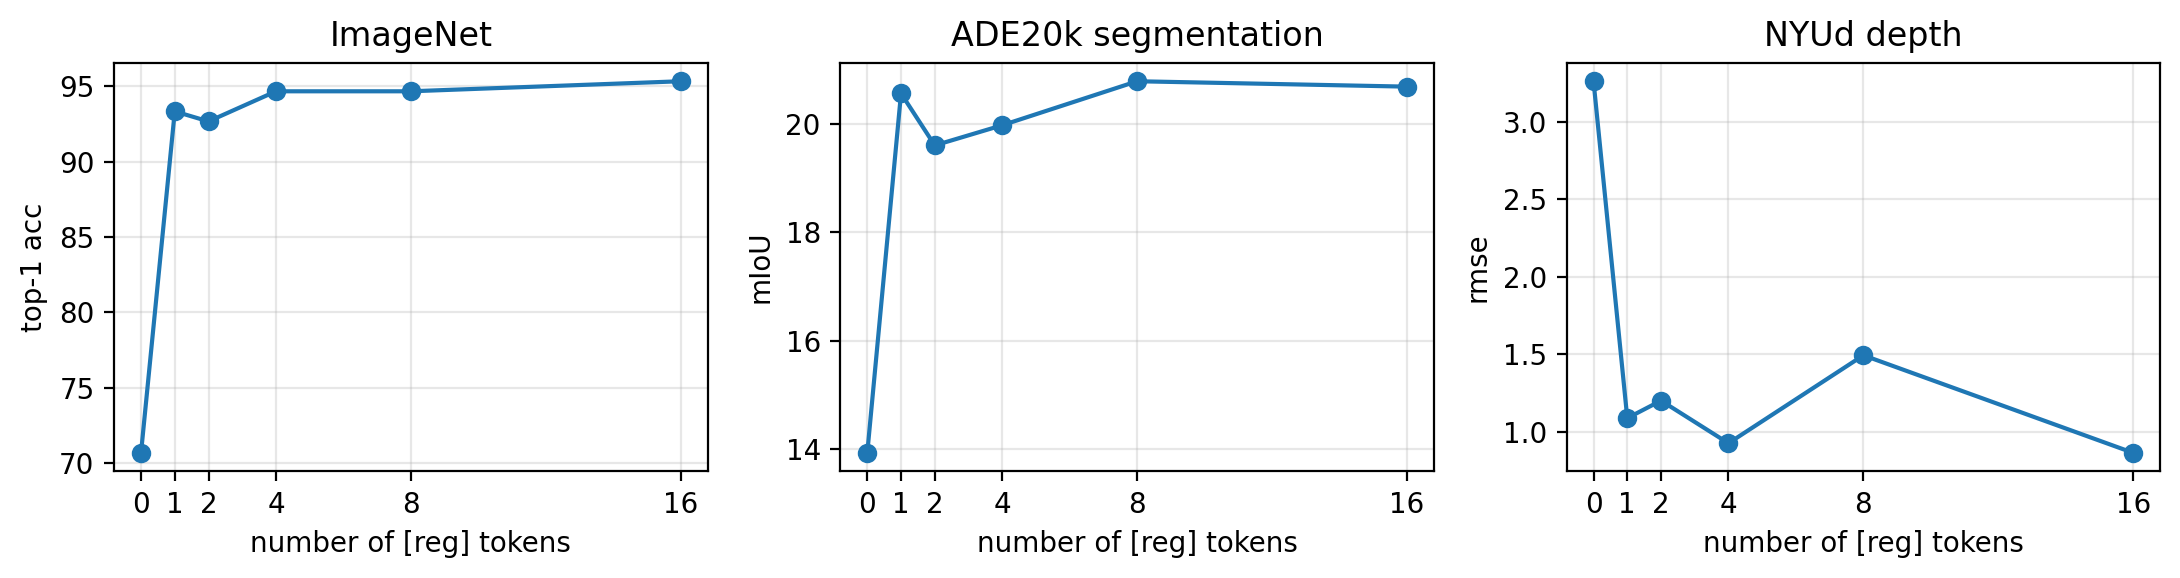
\includegraphics[width=0.95\linewidth]{../../src/Paolo/results/figure8_bottom.png}\\[2pt]
    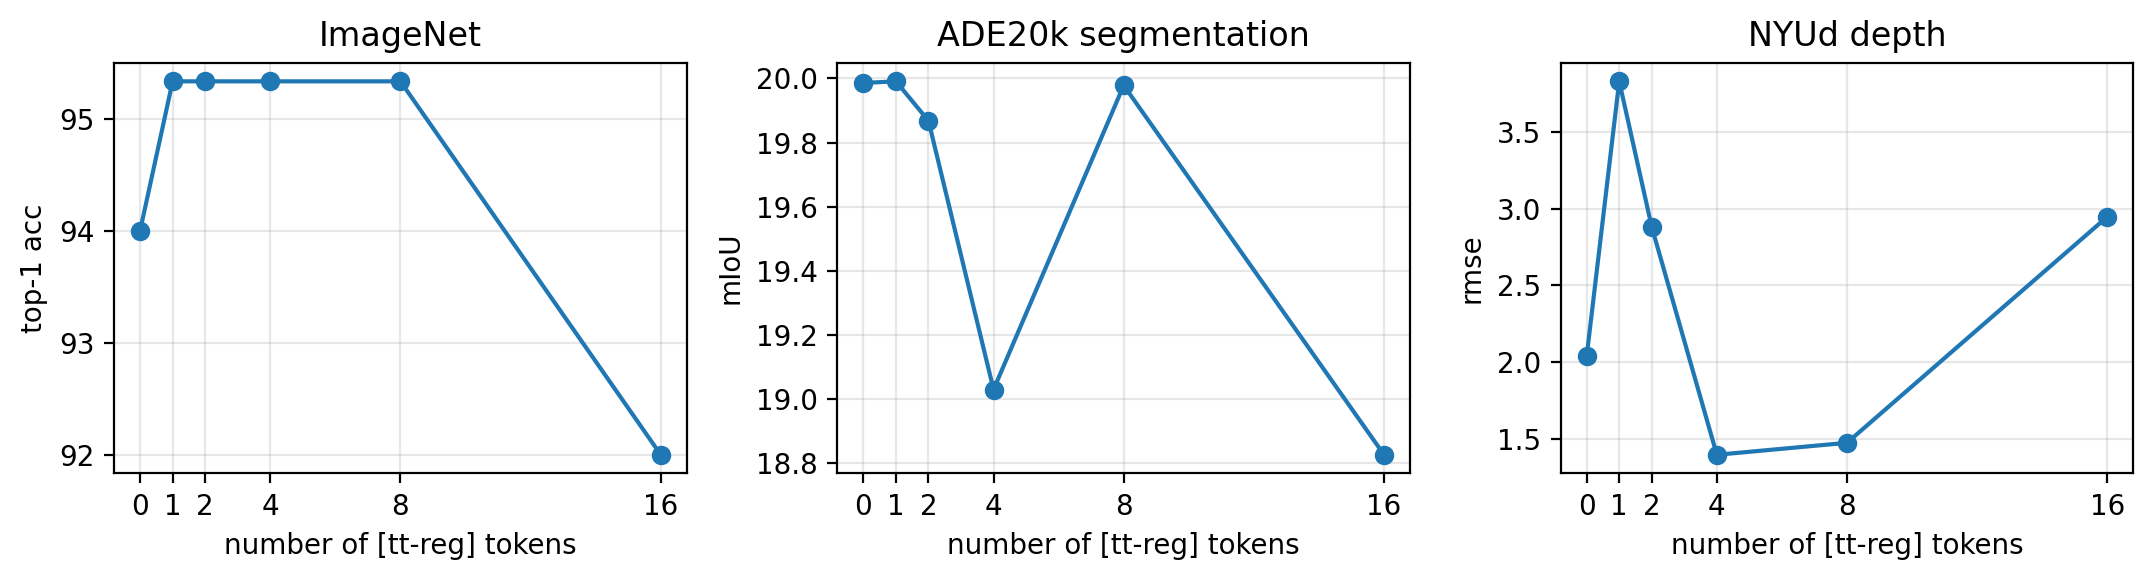
\includegraphics[width=0.95\linewidth]{../../src/Paolo/results/figure8_bottom_ttreg.png}\\[2pt]
    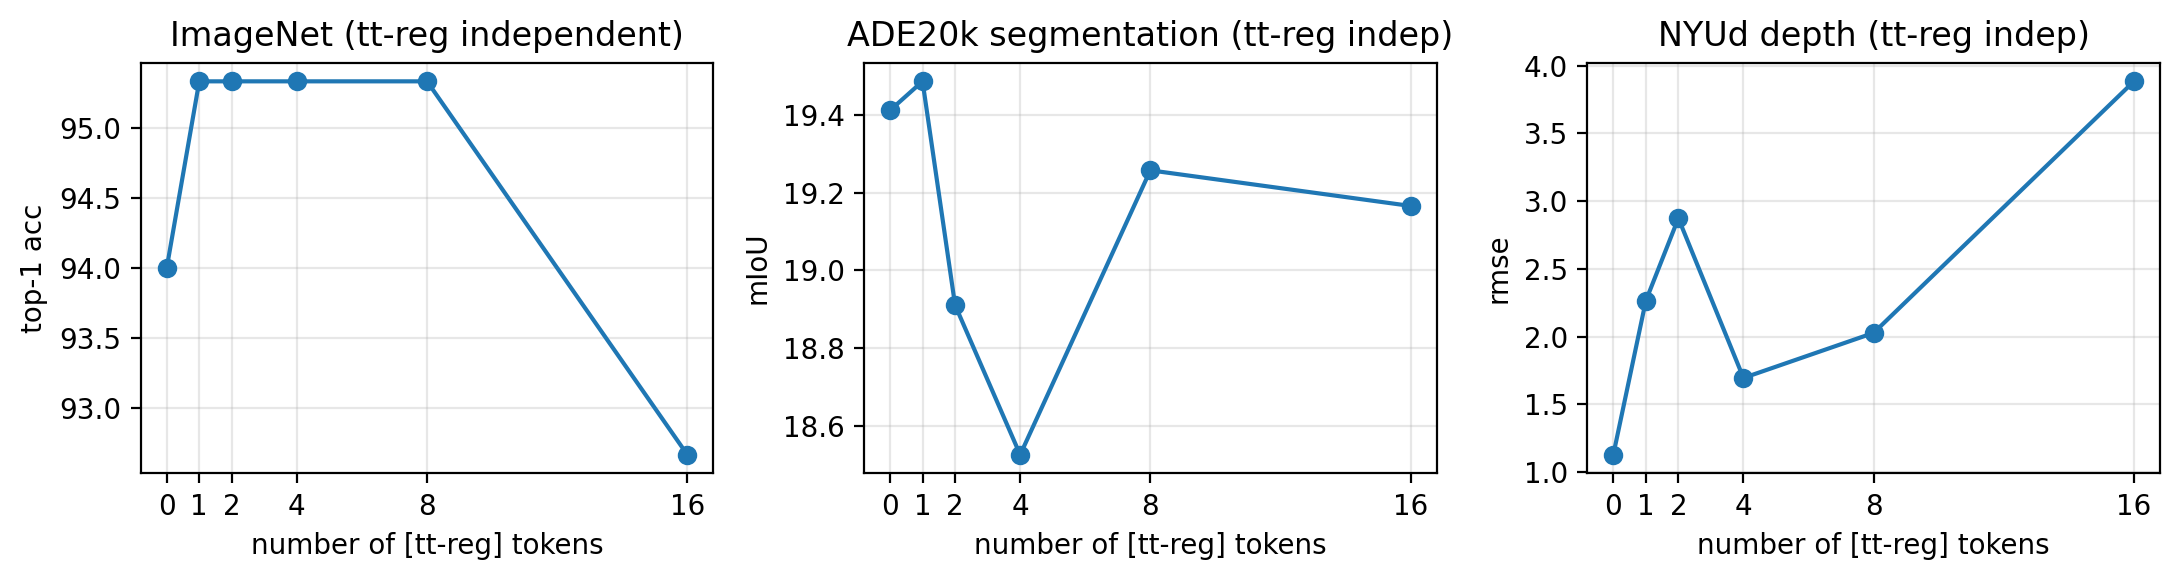
\includegraphics[width=0.95\linewidth]{../../src/Paolo/results/figure8_bottom_ttreg_indep.png}
    \caption{Downstream metrics (Top-1 on ImageNet, mIoU on ADE20k, RMSE on NYUd) as a function of the number of register tokens $N$. \textbf{Row 1}: truncate/cycle on DINOv2-reg4 -- near-binary behaviour, with $N=0$ catastrophic ($70.67\%$) and $N\geq 1$ plateauing around $94$--$95\%$. \textbf{Row 2}: Jiang test-time registers on the DINOv2 baseline -- a clean plateau at $95.33\%$ from $N=1$ to $N=8$, then a sharp collapse to $92.00\%$ at $N=16$. \textbf{Row 3}: our independent variant -- the same qualitative profile, falsifying the hypothesis that the $N=16$ collapse is caused by value duplication.}
    \label{fig:f8-bot}
\end{figure}

\begin{table}[H]
\centering
\caption{Figure~8 (bottom) numerical values for the two test-time register methods on DINOv2 ViT-L/14. Truncate/cycle values are reported in the main text.}
\label{tab:f8}
\begin{tabular}{ccccccc}
\toprule
& \multicolumn{3}{c}{\textbf{Jiang tt-reg}} & \multicolumn{3}{c}{\textbf{Independent variant}} \\
\cmidrule(lr){2-4}\cmidrule(lr){5-7}
$N$ & Top-1 & mIoU & RMSE & Top-1 & mIoU & RMSE \\
\midrule
0  & 94.00 & 19.99 & 2.04 m & 94.00 & 19.41 & 1.13 m \\
1  & 95.33 & 19.99 & 1.09 m & 95.33 & 19.49 & 2.26 m \\
2  & 95.33 & 19.87 & 1.20 m & 95.33 & 18.91 & 2.87 m \\
4  & 95.33 & 19.03 & 0.93 m & 95.33 & 18.53 & 1.69 m \\
8  & 95.33 & \textbf{19.98} & 1.49 m & 95.33 & 19.26 & 2.03 m \\
16 & 92.00 & 18.83 & 2.95 m & 92.67 & 19.17 & 3.88 m \\
\bottomrule
\end{tabular}
\end{table}
